\section{Common mistakes}

\begin{frame}{Image formats}
  \begin{columns}
    \begin{column}{0.5\textwidth}
      \begin{itemize}
        \item Do \emph{not} use \texttt{.jpeg} files for plots (
          \texttt{.jpeg} compresses text poorly)
        \item If you must use a raster format use \texttt{.png}
        \item Ideally use a vector format e.g. \texttt{.pdf}
      \end{itemize}
    \end{column}
    \begin{column}{0.5\textwidth}
      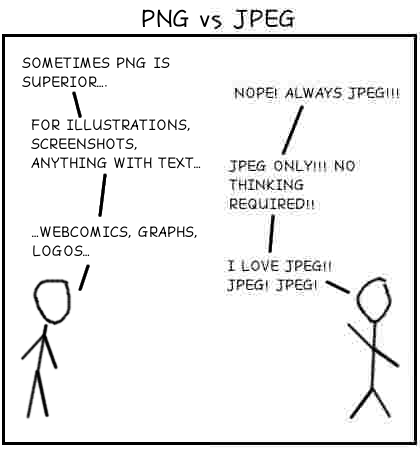
\includegraphics[width=0.85\textwidth]{jpg_vs_png.png}
    \end{column}
  \end{columns}
\end{frame}

\begin{frame}{Avoiding image scaling}
  \begin{itemize}
    \item Avoid scaling your plots using the \texttt{width} argument
      of \texttt{\tb includegraphics}
    \item Using \texttt{width} will scale the font sizes in your plot, making it
	  	difficult to control font size
	  \item Aim to create your plot with the \emph{exact} dimensions you need for
      your document
    \item The logic to achieve this is the same for whatever plotting software
      you use. \href{https://jwalton.info/Embed-Publication-Matplotlib-Latex/}%
      {Here} I outline an implementation for python.
  \end{itemize}
\end{frame}

\begin{frame}[fragile]{Typesetting maths}
  Brackets should be large enough to completely enclose all they contain.
  \begin{table}
    \centering
    \begin{tabular}{cl}
      $(\sum\limits_{i=1}^{n-1} i) + n$ \hspace{1cm} &
        \lstinline|(\sum_{i=1}^{n-1} i) + n| \\ & \\
      $\bigg(\sum\limits_{i=1}^{n-1} i\bigg) + n$ \hspace{1cm} &
        \lstinline|\bigg( \sum_{i=1}^{n-1} i \bigg) + n| \\
    \end{tabular}
  \end{table}
\end{frame}

\begin{frame}[fragile]{Typesetting maths}
  \begin{table}
    \centering
    \begin{tabular}{ll}
      \color{red}\lstinline|$a, b, c, d, e \text{ and } f$| \hspace{1cm} &
        \color{red}$a, b, c, d, e \text{ and } f$ \\ & \\
      \color{mLightGreen}\lstinline|$a$, $b$, $c$, $d$, $e$ and $f$| &
        \color{mLightGreen}$a$, $b$, $c$, $d$, $e$ and $f$\hspace{1cm}\\& \\
      \color{red}\lstinline|$i=1,...,10$| &
        \color{red}$i=1,...,10$ \\ & \\
      \color{mLightGreen}\lstinline|$i=1,\ldots,10$| &
        \color{mLightGreen}$i=1,\ldots,10$ \\ & \\
      \color{red}\lstinline|$sin(x)^2 + cos(x)^2 = 1$| &
        \color{red}$sin(x)^2 + cos(x)^2 = 1$ \\ & \\
      \color{mLightGreen}\lstinline|$|\tb\lstinline|sin(x)^2 + |
        \tb\lstinline|cos(x)^2 =1|\lstinline|$| &
        \color{mLightGreen}$\sin(x)^2 + \cos(x)^2 = 1$ \\
    \end{tabular}
  \end{table}
\end{frame}

\begin{frame}[fragile]{Hyphen, en-dash and em-dash (-, --, ---)}
  \begin{itemize}
    \item The \textcolor{mLightGreen}{hyphen} (\lstinline|-|) is used to join
      words in a compound construction. ``A long-term solution''
    \item An \textcolor{mLightGreen}{en-dash} (\lstinline|--|) appears in page
      ranges. ``See pages 1--3''
    \item An \textcolor{mLightGreen}{em-dash} (\lstinline|---|) is typically
      used as a stand-in for a comma or parenthesis to separate out phrases.
      ``Against all odds, Boris --- the class clown --- became prime minister.''
  \end{itemize}
\end{frame}

\begin{frame}[fragile]{Quotes}
  \LaTeX\ requires you to use separate markup for opening and closing quotes. 

  Opening quotes are \lstinline|``|

  Closing quotes are \lstinline|''|

  Quotes should look ``like this'' not ''like this''.
\end{frame}

\begin{frame}[fragile]{Capitalisation in BibTeX}
  Your BibTeX style will handle most capitalisation. For some words (names,
  places, \ldots) capitalisation must be ensured
  \begin{lstlisting}
@book{springer57,
  title="Introduction to {R}iemann surfaces",
  author="Springer, George",
  volume="473",
  year="1957",
  publisher="Addison-Wesley Reading"
}
  \end{lstlisting}
\end{frame}

